\documentclass[a4paper]{article}
\usepackage[a4paper,  margin=1.0in]{geometry}

\usepackage{graphicx}
\usepackage{float}
\usepackage{hyperref}
\usepackage{listings}
\lstset{
basicstyle=\small\ttfamily,
columns=flexible,
breaklines=true
}

\usepackage{polski}
\usepackage[utf8]{inputenc}
\begin{document}


\title{Ćwiczenie nr 2 z MBI, adnotacja DNA}
\author{Mateusz Chydziński, Michał Sypetkowski}
\maketitle

\section{Ogólne informacje}
Repozytorium git: \url{https://github.com/msypetkowski/MBI-exercises.git}.
W katalogu \texttt{cw2} repozytorim zawiera skrypty/polecenia użyte do przeprowadzenia eksperymentów.

\section{Przygotowanie danych}
Cały przykładowym genom zawiera 3035 kontigów fizycznych.
Do badań wykorzystany został kontig fizyczny o identyfikatorze:
\begin{verbatim}
>HDID_scaffold0000001 length=355889
\end{verbatim}

\section{Maskowanie genomu}
Ilość nukleotydów, która została zamaskowana w wyniku działania programu RepeatMasker:
\begin{verbatim}
2478
\end{verbatim}

\section{Mapowanie znanych sekwencji i adnotacja strukturalna}
Pierwsze 10 linii z logu programu maker:
\begin{lstlisting}
##gff-version 3
HDID_scaffold0000001	.	contig	1	355889	.	.	.	ID=HDID_scaffold0000001;Name=HDID_scaffold0000001
###
HDID_scaffold0000001	repeatmasker	match	7846	9011	1224	+	.	ID=HDID_scaffold0000001:hit:0:1.3.0.0;Name=species:Mariner-6_ACe|genus:DNA%2FTcMar-Tc1;Target=species:Mariner-6_ACe|genus:DNA%2FTcMar-Tc1 1 1094 +
HDID_scaffold0000001	repeatmasker	match_part	7846	9011	1224	+	.	ID=HDID_scaffold0000001:hsp:0:1.3.0.0;Parent=HDID_scaffold0000001:hit:0:1.3.0.0;Target=species:Mariner-6_ACe|genus:DNA%252FTcMar-Tc1 1 1094 +
HDID_scaffold0000001	repeatmasker	match	42975	43896	707	+	.	ID=HDID_scaffold0000001:hit:1:1.3.0.0;Name=species:Mariner-6_CFl|genus:DNA%2FTcMar-Mariner;Target=species:Mariner-6_CFl|genus:DNA%2FTcMar-Mariner 262 1175 +
HDID_scaffold0000001	repeatmasker	match_part	42975	43896	707	+	.	ID=HDID_scaffold0000001:hsp:1:1.3.0.0;Parent=HDID_scaffold0000001:hit:1:1.3.0.0;Target=species:Mariner-6_CFl|genus:DNA%252FTcMar-Mariner 262 1175 +
HDID_scaffold0000001	repeatmasker	match	162805	163521	673	+	.	ID=HDID_scaffold0000001:hit:2:1.3.0.1;Name=species:Mariner-43_HSal|genus:DNA%2FTcMar-Mariner;Target=species:Mariner-43_HSal|genus:DNA%2FTcMar-Mariner 494 1199 +
HDID_scaffold0000001	repeatmasker	match_part	162805	163521	673	+	.	ID=HDID_scaffold0000001:hsp:2:1.3.0.1;Parent=HDID_scaffold0000001:hit:2:1.3.0.1;Target=species:Mariner-43_HSal|genus:DNA%252FTcMar-Mariner 494 1199 +
HDID_scaffold0000001	repeatmasker	match	163678	163840	231	+	.	ID=HDID_scaffold0000001:hit:3:1.3.0.1;Name=species:Mariner-25_HSal|genus:DNA%2FTcMar-Mariner;Target=species:Mariner-25_HSal|genus:DNA%2FTcMar-Mariner 185 347 +
\end{lstlisting}

\section{Adnotacja funkcjonalna}
Znaleziony w pliku .gff identyfikator sekwencji:
\begin{lstlisting}
HDID_scaffold0000001	blastn	expressed_sequence_match	17669	18426	40	-	.	ID=HDID_scaffold0000001:hit:16:3.2.0.0;Name=HDID_0000675501-mRNA-1
\end{lstlisting}

Nukleotydy w tej sekwencji to:

\begin{verbatim}
TAAAATCCAGAACAACAAGCCTTTTTCGGTTGGTTACTGTCCTGTTGGAGAGGAATAGTA
GGCTTACTGCCCAATGGAAGGGCATTATTGGAATTCACGGAGGGTGTTCCTACAATTTTA
AGAATATCTTAACAAAAATCGCACTTGAAAAGTAGTCCTTACCTTCAAGAAGGGTGGAAA
AAGCTCGATCGACATTGGTTGAGTCTAAGGCTGATGTTTCAATGAAGTGAAGACAAGTAT
CTTCAGCGAATTGCTTGGCTTCTTGCGTAGAAACCGTACGCAGATGGCGCAGATCACATT
TATTTCCAACTAATATGGTGACAATATTTCGATCAGCATTATTCTTAAGTTCCTTCAACC
ATACGTTCACATTTTCAAAAGTAGTGTACTTAGCTATATCATATACAAGCAGAGCTCCAA
CAGCACCGCGATAATACCTATAGAAAACAGAACTAATTATAGAAAAATACTCAACTTACG
CTGACGTTATTGCTCTGTATCTTTCTTGGCCGGCTGTATCCCAAATTTGGATTTTTATAA
CCTTATCACCTATCTTAACACTCCTGGTTGCGAATTCAACGCCGATTGTGGTTTTACTCT
CCAAGTTAAATTGATTACGAGTGTATCGAGAGAGTAGATTGCTCTTACCGACACCTGAAT
CCCCTATTAATACGACTAAAATATATAAGAAATGATTAATTAAAAGAAAATAAATACTTT
TGAAAAGGTAATCATATGAATCTTCATCGTTGGCCAT
\end{verbatim}

\begin{figure}[h]
    \centering
    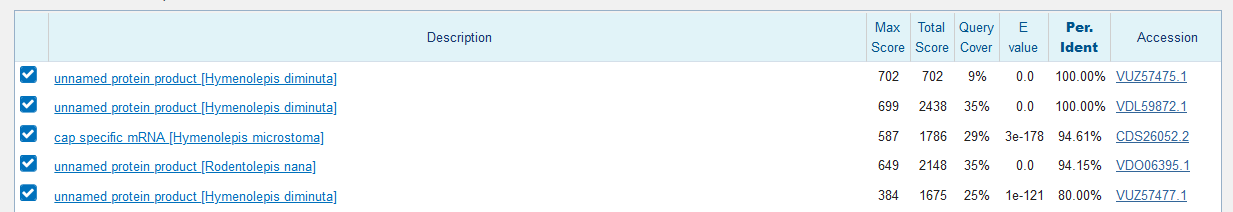
\includegraphics[width=1.0\textwidth]{result.png}
    \label{fig:single}
    \caption[]{Wyniki z blastx}
\end{figure}

\section{Adnotacja funkcjonalna}
Genom użyty w badaniu należy do organizmu \texttt{hymenolepis diminuta}, czyli tasiemca szczurzego. Analiza podobieństwa sekwencji za pomocą 
algorytmu BlastX została przeprowadzaona dla scaffoldu pierwszego, o oznaczeniu \texttt{HDID\_scaffold0000001}. W wyniku działania algorytmu
zostały znalezione 4 sekwencje podobne, o znacznym stopniu podobieństwa (94\% dla 1 sekwencji oraz 100\% dla 3 pozostałych). Istotność wyniku 
\texttt{E-value} jest na poziomie około \texttt{0.004}, co spełnia warunek \texttt{E<<1} i sprawia, że prawdopobieństwo przypadkowego dopasowania
sekwencji źródłowej do znalezionych jest bardzo małe. Pierwszy wynik na liście potwierdza, że jest to rzeczywiście poprawny scaffold tego organizmu
(stopień podobieństwa 100\% oraz E-value=0). Ponadto stwierdzono duży stopień podobieństwa sekwencji do \texttt{Candida dubliniensis} - odmiany
patogennego grzyba (sekwencja kodująca jedno z białek oraz chromosom nr.1). Ostatnim wpisem na liście wyników jest jedno z białek orgaznizmu
\texttt{chenopodium quinoa}, czyli rośliny - komosy ryżowej. 

\end{document}
